\documentclass[tikz,border=3pt]{standalone}
\usepackage[utf8]{inputenc}
\usepackage[T1]{fontenc}
\usepackage{lmodern}
\renewcommand{\familydefault}{\sfdefault}
\usepackage{sansmath}\sansmath
\usepackage{chemfig}
\usepackage{pgfplots}\pgfplotsset{compat=1.18,/pgf/number format/use comma,/pgf/number format/1000 sep={.}}
\usetikzlibrary{arrows.meta,calc,positioning,decorations.pathmorphing,patterns}
% paleta del sitio
\definecolor{nar}{HTML}{E8680C}\definecolor{narc}{HTML}{FFB35C}\definecolor{hielo}{HTML}{FFF3E8}
\definecolor{tinta}{HTML}{1D1D1F}\definecolor{gris}{HTML}{6E6E73}\definecolor{lila}{HTML}{7C5CF0}
\definecolor{azul}{HTML}{2F6FD6}\definecolor{menta}{HTML}{17A673}\definecolor{coral}{HTML}{E8342A}
\begin{document}
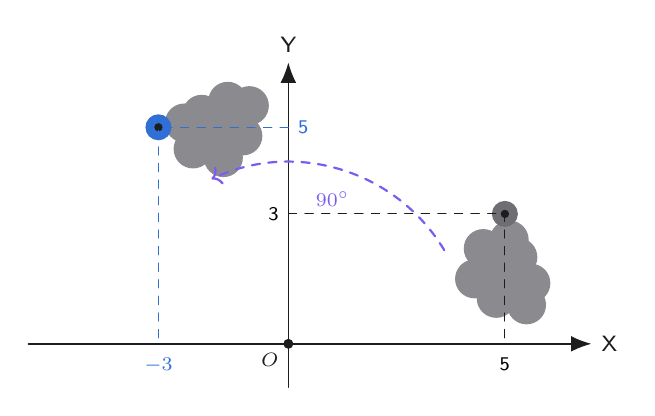
\begin{tikzpicture}[font=\small,x=0.55cm,y=0.55cm,line cap=round,line join=round,step={(1,1)}]
\fill[gris!80] (4.50,2.20) circle (0.45);
\fill[gris!80] (5.30,2.00) circle (0.45);
\fill[gris!80] (4.90,1.60) circle (0.45);
\fill[gris!80] (4.30,1.50) circle (0.45);
\fill[gris!80] (5.60,1.40) circle (0.45);
\fill[gris!80] (5.10,2.40) circle (0.45);
\fill[gris!80] (4.80,1.05) circle (0.45);
\fill[gris!80] (5.50,0.90) circle (0.45);
\fill[gris!80] (-2.20,4.50) circle (0.45);
\fill[gris!80] (-2.00,5.30) circle (0.45);
\fill[gris!80] (-1.60,4.90) circle (0.45);
\fill[gris!80] (-1.50,4.30) circle (0.45);
\fill[gris!80] (-1.40,5.60) circle (0.45);
\fill[gris!80] (-2.40,5.10) circle (0.45);
\fill[gris!80] (-1.05,4.80) circle (0.45);
\fill[gris!80] (-0.90,5.50) circle (0.45);
\draw[-{Latex[length=2.6mm,width=2mm]},tinta,semithick] (-6,0)--(7,0) node[right,font=\footnotesize] {X};
\draw[-{Latex[length=2.6mm,width=2mm]},tinta,semithick] (0,-1)--(0,6.5) node[above,font=\footnotesize] {Y};
\fill[gris] (5,3) circle (0.3); \fill[tinta] (5,3) circle (1.5pt);
\fill[azul] (-3,5) circle (0.3); \fill[tinta] (-3,5) circle (1.5pt);
\draw[dashed,tinta] (0,3)--(5,3)--(5,0);
\draw[dashed,azul] (0,5)--(-3,5)--(-3,0);
\node[left,font=\scriptsize] at (0,3) {3}; \node[below,font=\scriptsize] at (5,-0.1) {5};
\node[right,font=\scriptsize,text=azul] at (0,5) {5}; \node[below,font=\scriptsize,text=azul] at (-3,-0.1) {$-3$};
\draw[lila,thick,dashed,->] (31:4.2) arc (31:115:4.2);
\node[font=\scriptsize,text=lila] at (73:3.5) {$90^\circ$};
\fill[tinta] (0,0) circle (1.8pt) node[below left,font=\scriptsize] {$O$};
\end{tikzpicture}
\end{document}
